The code resides in src/cuda/ and only minor changes have been made to the original MarDyn code. These changes will be described in great detail later as well.

The \cuda{} code moves the molecule interaction calculation to the GPU. It calculates the interactions between different molecules using different potential models as specified in the component description\TODO{reference to Mardyn docs}.
A \cuda{} application performs basically three steps:
\begin{compactenum}
\item upload data to the GPU
\item process data on the GPU
\item download results from the GPU
\end{compactenum} 
Different information has to be uploaded in MarDyn. Information about the different molecule types (\textbf{component descriptions}) has to be uploaded only once. The position and orientation of every molecule has to be uploaded for each force calculation. 
Later the calculated forces and torque have to be downloaded, as well as the calculated potential and virial statistics.

The Linked Cells-algorithm is used in MarDyn. The simulation space is divided into cells and the interaction between molecules of the same and of neighboring cells have to be calculated.
This leads to a natural parallelization approach:
\begin{compactitem}
\item for \textbf{intra-cell molecule interactions} each thread can process the molecules of one cell, and
\item for \textbf{inter-cell molecule interactions} each thread can process a different pair of neighboring cells.
\end{compactitem}

\subsection{General Architecture}
The \cuda{} coda is split up in different components. Each component has exactly one responsibility.
The intention to make it clear where changes go and make it easier to navigate the code.

A \textbf{component} usually consists of CPU and \cuda{} code which interact somehow. For this there usually are a \filename{component.cpp} and \filename{component.h}, which contain the CPU-side code, and a \filename{component.cum}, which contains the \cuda{} code\footnote{\filename{.cum} stands for \textbf{cu}da \textbf{m}odule}.

Normally you pass parameters as kernel parameters to \cuda{}. Separation of responsibilities is the main goal of having different components. Thus passing all paramaters as kernel parameters is not a good approach. The CPU code of each component needs a way to interact with the \cuda{} code and the 'glue' code should be part of the components and not be kept somewhere else\footnote{the first implementation used kernel parameters and the parameter count quickly became unacceptable}.

The solution is simple: \cuda{} supports global variables and the CPU/\cuda{} interface in each component uses global variables to exchange data\footnote{using a different namespace for each component would be preferable to guarantee no naming conflicts}.

Moreover, instead of global variables constant\footnote{\TODO{see the Cuda docs!}} variables could be used, which reside in constant memory. Constant memory has its own on-chip cache, so this is desirable, too\footnote{generally speaking, the more cache memory can be used, the better the preformance}.

\begin{figure}
\caption{Components and \cuda{} modules}
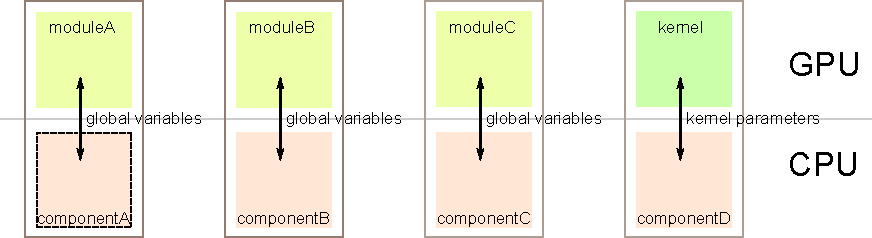
\includegraphics{figures/component_architecture.pdf}
\end{figure}
\TODO{add diagrams showing the architectural principles and code examples}

\subsection{Component Overview}
Most components implement a \lstinline!CUDAComponent! interface. There are two of them:
\begin{compactitem}
\item \lstinline!CUDAForceCalculationComponent! is used by components that perform data exchange operations on each force calculation, and
\item \lstinline!CUDAStaticDataComponent! is used by components that only need to upload data once.
\end{compactitem}

There are quite a few different components:
\begin{compactdesc}
\item[CellProcessor] contains logic to efficiently loop through the molecules of a single cell or a cell pair
\item[ComponentDescriptor] manages the molecule component descriptions such as how many Lennard-Jones centers a molecule has.
\item[MoleculeInteraction] links all components together and calculates the forces
\item[GlobalStats] keeps track of the total potential and virial statistics
\item[MoleculePairHandler] calculates the force between two given molecules
\item[MoleculeStorage] manages all per-molecule data like positions, forces or orientations
\item[PairTraverser] enumerates all cell pairs in a way that allows for maximum parallelization
\item[PotForce] calculates the force between Lennard-Jones centers, dipoles, etc
\end{compactdesc}

\begin{figure}
\caption{Component dependencies}
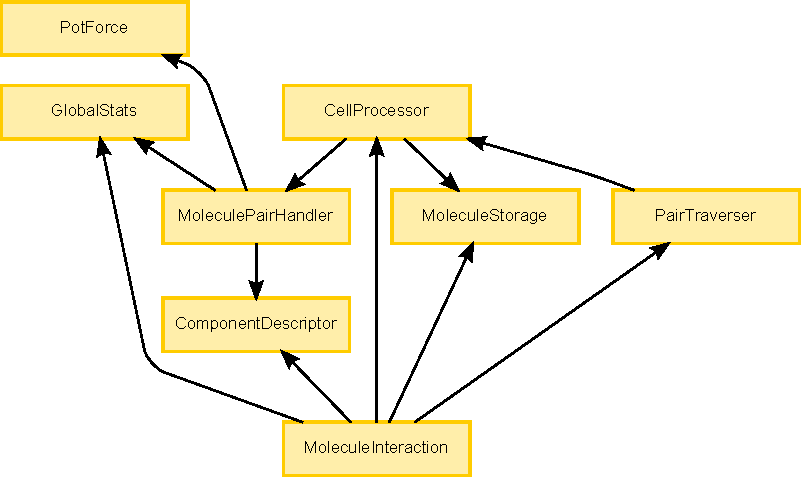
\includegraphics{figures/component_dependencies.pdf}
\end{figure}

There are additional \cuda{} modules that contain helper and utility functions.
All the \filename{.cum} files are included in \filename{kernel.cu}, which also contains the two kernel entrance functions \lstinline!processCellPair! and \lstinline!processCell!, which are called by \textbf{MoleculeInteraction} to calculate the forces between all the molecules in a cell pair or in a single cell.

\subsection{\cuda{} Helper Classes and Functions}
\filename{helpers.cpp/h} contain C++ wrappers for all \cuda{} functionality that is used in the project.
It implements an in-language DSL\footnote{domain-specific language} to simplify working with the \cuda{} API.

\TODO{add class diagram of helpers.h}

\subsubsection{Device Buffers and Global Variables}
Managing device memory is done by creating instances \lstinline!CUDA::DeviceBuffer<DataType>!. Methods are provided to resize the buffer and to copy data from and to the GPU.
Global variables are mapped to \lstinline!CUDA::Global<DataType>! objects. They provide a \lstinline!set! method that is specialized for pointer global variables to take \lstinline!CUDA::DeviceBuffer<DataType>! objects.
Example:
\begin{lstlisting}[label=cudamemoryhelpers,caption=CUDA helper classes for Device Memory and Globals]
class GlobalStats : public CUDAForceCalculationComponent {
	CUDA::Global<CellStatsStorage *> _cellStats;
	CUDA::DeviceBuffer<CellStatsStorage> _cellStatsBuffer;
	
	GlobalStats( const CUDAComponent &component ) :
		_cellStats( _module.getGlobal<CellStatsStorage *>("cellStats") )
	/* ... */
	
		_cellStatsBuffer.resize( _linkedCells.getCells().size() );
		_cellStatsBuffer.zeroDevice();
		_cellStats.set( _cellStatsBuffer );		
	/* ... */		
};	
\end{lstlisting}

\subsubsection{Calling \cuda{} Functions}
The \lstinline!Function! class wraps \cuda{} functions. It has a \lstinline!call! method that returns a \lstinline!FunctionCall! object that can be used to specify the grid and block sizes and parameters before running the \cuda{} kernel by calling its \lstinline!execute! method.
Example:
\begin{lstlisting}[label=cudafunctionhelpers,caption=CUDA helper classes for Function Calls]
	CUDA::Function _convertQuaternionsToRotations;
/* ... */		
	MoleculeStorage( const CUDAComponent &component ) :
		_convertQuaternionsToRotations( _module.getFunction( "convertQuaternionsToRotations" ) )
/* ... */
		_convertQuaternionsToRotations.call().
			parameter(quaternionBuffer.devicePtr()).
			parameter(currentIndex).
			setBlockShape(MAX_BLOCK_SIZE, 1, 1).
			execute(currentIndex / MAX_BLOCK_SIZE + 1, 1);
\end{lstlisting}

\subsubsection{\filename{cutil\_double\_math.h}}
The \cuda{} SDK provides a helper file called \filename{cutil\_math.h} which adds overloaded operators and functions for most \cuda{} datatypes except \lstinline!double2!, \lstinline!double3! and \lstinline!double4!.
\filename{cutil\_double\_math.h} adds support for these datatypes.
This makes it possible to switch between single- and double-precision using a simple preprocessor \#define.

\subsubsection{Pair Traverser}
The simulation space is divided into a grid of cells. \TODO{add picture} The pair traverser iterates over all neighbors pairings in the volume while maximizing parallelism. Each cell inside the volume has 26 neighbors. There are 13 directions, so that two neighbors always lie on a line. It doesn't matter if you calculate the interactions between cell A and B or cells B and A. This symmetry allows for a straight-forward parallelization.
I am going to introduce it using the special case of the direction along the x-axis:
\begin{compactenum}
\item calculate the interactions between all cells $ \left ( 2*k, y, z \right ) $ and $ \left ( 2*k + 1, y, z \right ) $ in parallel (even case)
\item calculate the interactions between all cells $ \left ( 2*k + 1, y, z \right ) $ and $ \left ( 2*k + 2, y, z \right ) $ in parallel (odd case)
\end{compactenum}
It's easy to see that this covers all neighbor pairings along the x-axis. \TODO{add picture}
The algorithm takes the even or odd layers parallel to the yz-plane and computes the interaction with the neighboring cells.

All other directions can be treated like this. You only have to make sure that the boundaries are not invalidated.

The cells are flattened into a one-dimensional array and the CPU code calculates:
\begin{compactitem}
\item the index of the first cell (\lstinline!startIndex!)
\item the size of the two-dimensional grid that constitutes the parallel layers (\lstinline!dimension!)
\item offsets to move in x-, y- and z-direction in the one-dimensional cell array, whereas this constitutes a local coordinate system, such that the x- and y- span the two-dimensional grid and z- moves along the layers (\lstinline!gridOffsets!)
\item offset to get the neighbor cell for a cell (\lstinline!neighborOffset!)
\end{compactitem}
With these parameters, the \lstinline!processCellPair! kernel can be launched with $ \text{dimension} \times     \text{number of layers} $ thread blocks\footnote{one thread block per cell pair}.

\subsubsection{Molecule Storage}
The molecule storage component manages everything related to molecule data. The molecules of all the cells are flattened into a one-dimensional array. For each cell the start index into this array is stored in a \lstinline!cellStartIndices! array. \TODO{add picture}

The molecule data such as position, orientation, total force and torque, and molecule type, are stored non-interleaved into different buffers: \lstinline!moleculePositions!, \lstinline!moleculeRotations!, \lstinline!moleculeForces!, \lstinline!moleculeTorque! and \lstinline!moleculeComponentTypes!.

The molecule orientation is stored and uploaded as quaternions, but converted to conventional $ 3 \times 3 $-matrices on the GPU.

The \cuda{} code wraps accesses to the data through a \lstinline!MoleculeStorage! class, which has \lstinline!get! and \lstinline!set! methods, which operate on a \lstinline!Molecule! structure. So the abstraction is that the data is interleaved or rather stored as an array of \lstinline!Molecule!s. This makes it possible to write the molecule interaction code without having to care for the actual implementation.

There is also a \lstinline!MoleculeLocalStorage<blockSize>! class. It provides a cache for frequently used molecules. Its objects are supposed to be instanciated as \lstinline!__shared__! objects and there are methods to load, merge and commit molecules from the cache to the regular storage.

\subsubsection{Global Statistics}
The potential and virial are calculated per cell on the GPU. For this the CPU code creates shared arrays for one potential and one virial value per thread in a threadblock, so the values can be updated by their threads without locks. The \lstinline!CellStatsCollector! class has a \lstinline!reduceAndSave! which sum-reduces the two arrays into a cell potential and cell virial values.

The CPU code then reduces these per-cell values into per-domain values. Potentials and virials are calculated per molecule pair and added to the cells the molecules belong to\footnote{in the case of molecules from the same cell, the values are added to the same cell twice}. Now the domain values, as sum of call cell values, count each potential and virial twice, so the code halves the values.

There is also an implementation difference to the regular MarDyn code: the force interaction code in MarDyn defines \lstinline!distanceAtoB! as \lstinline!positionA - positionB!, while the \cuda{} code defines it as \lstinline!positionB - positionA!\footnote{which makes more sense sementically}. Because of this sign change, the calculated GPU virial has to be sign inverted, too, to match the CPU virial value.

\subsubsection{Cell Processor}
The cell processor processes all molecules in the same cell (intra-cell) or between two cells (intra-cell).
The reference approach is to iterate through all molecule pairs in both cells and calculate the interactions between them:
\begin{figure}
  \centering
  \subfloat[First eight molecule interactions]{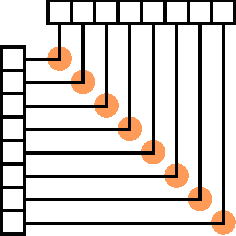
\includegraphics[width=0.3\textwidth]{figures/cellprocessor_first_iteration.pdf} }                
  \subfloat[All inter-cell interactions]{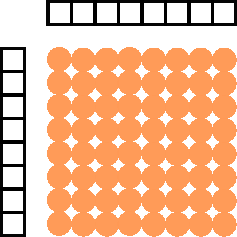
\includegraphics[width=0.3\textwidth]{figures/cellprocessor_all_iterations_inter_cell.pdf} }
  \subfloat[All intra-cell interactions]{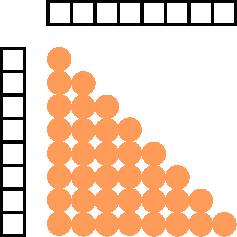
\includegraphics[width=0.3\textwidth]{figures/cellprocessor_all_iterations_intra_cell.pdf}}
  \caption{Schematic of molecule interactions between two cells}
\end{figure}

\begin{lstlisting}[label=intercellreferenceloop,caption=Reference Inter-Cell Block Processing]
__device__ void processCellPair(const int threadIndex, const CellInfo & cellA, const CellInfo & cellB) {
	for( int indexA = cellA.startIndex ; indexA < cellA.endIndex ; indexA++ ) {
		Molecule moleculeA;
		moleculeDataAccessor.get( indexA, moleculeA );
		for( int indexB = cellB.startIndex ; indexB < cellB.endIndex ; indexB++ ) {
			Molecule moleculeB;
			moleculeDataAccessor.get( indexB, moleculeB );

			moleculePairHandler.process( 0, moleculeA, moleculeB );

			moleculeDataAccessor.set( indexB, moleculeB );
		}
		moleculeDataAccessor.set( indexA, moleculeA );
	}
}
\end{lstlisting}
The intra-cell code is similar. The only difference is that only half of the interactions have to be calculated, because of the order\footnote{molecule A with molecule B is the same as molecule B with molecule A} does not matter:
\begin{lstlisting}[label=intracellreferenceloop,caption=Reference Intra-Cell Block Processing]
__device__ void processCell(const int threadIndex, const CellInfo & cell) {
	for( int indexA = cell.startIndex ; indexA < cell.endIndex ; indexA++ ) {
		Molecule moleculeA;
		moleculeDataAccessor.get( indexA, moleculeA );
		for( int indexB = cell.startIndex ; indexB < indexA; indexB++ ) {
			Molecule moleculeB;
			moleculeDataAccessor.get( indexB, moleculeB );

			moleculePairHandler.process( 0, moleculeA, moleculeB );

			moleculeDataAccessor.set( indexB, moleculeB );
		}
		moleculeDataAccessor.set( indexA, moleculeA );
	}
}
\end{lstlisting}

The main idea in the parallelized approach is to divide the cells into smaller blocks that can be kept in shared memory and process interactions inside between the different blocks. Parallelized matrix multiplication is based on the same idea. \TODO{see cuda reference}

Thus the fast cell processor divides the cells into blocks. Each block contains one molecule per thread in a thread block.
The code then iterates over all block pairs in both cells and calculates the interactions between molecules of the two blocks.
The inter-cell case is straight-forward:
\begin{lstlisting}[label=intercellloop,caption=Inter-Cell Block Processing]
for( int blockIndexA = 0 ; blockIndexA < numBlocksA ; blockIndexA++ )
	for( int blockIndexB = 0 ; blockIndexB < numBlocksB ; blockIndexB++ )
		processBlock<BPT_UNRELATED>( /* ... */ );

\end{lstlisting}
For the intra-cell case only half of the block pairs have to be processed, because again it does not matter if block A with block B are processed of vice-versa:
\begin{lstlisting}[label=intracellloop,caption=Intra-Cell Block Processing]
for( int blockIndexA = 0 ; blockIndexA < numBlocksA ; blockIndexA++ ) {
	processBlock<BPT_SAME_BLOCK>( /* ... */ );
	
	for( int blockIndexB = 0 ; blockIndexB < blockIndexA; blockIndexB++ )
		processBlock<BPT_UNRELATED>( /* ... */ );
}
\end{lstlisting}
Likewise, the calculation of interactions inside the same block (ie intra-block) have to be treated as special case.

There is one molecule per thread in a thread block in each block. Since there are as many threads as molecules in a block, each thread can be assigned a fixed molecule of block A (outer block loop). This molecule can be stored in registers or in local memory.
The molecules of block B (inner block loop) can be stored in shared memory, since they are only accessed by diffferent threads of the same thread block.

\begin{figure}
\caption{Schematic of one block iteration (with a thread blocks of size 8 and warps of size 4, and all 8 parallel molecule pair iterations are shown for the block pair)}
\centering
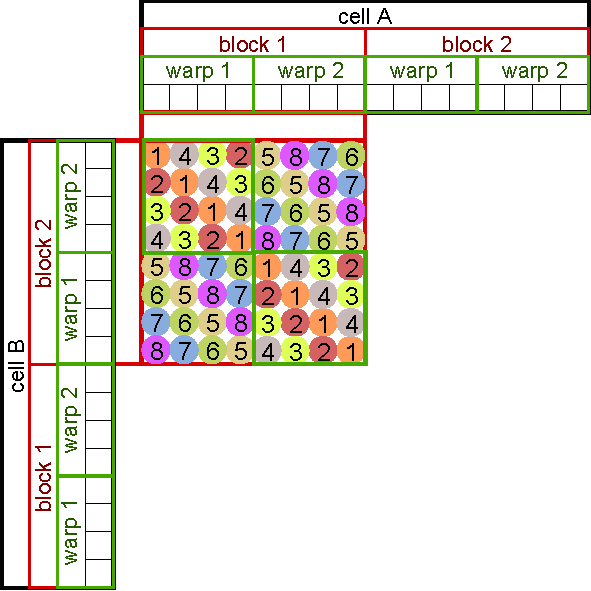
\includegraphics{figures/cellprocessor_block_iteration_1.pdf}
\end{figure}

Straight-forward block processing would simply loop over all molecules in block B and each thread would calculate the interactions of its fixed molecule from block A with one molecule from block B.
Again this is not the best solution. Instead a block is divided into \textbf{warp-blocks}. Each warp-block contains 32 molecules\footnote{exactly the warp size}.
The aim here is not to improve cache usage, but to require less explicit synchronization.
In the naive approach there would have to be a barrier after each interaction calculation to make sure that each thread is done with processing its molecule pair because another thread will access the molecule from block B in shared memory next.
Threads in the same warp are synchronized by design, because they are executed in lockstep, so processing  molecule interactions warp-block by warp-block improves parallelism.
Again there is a special case when interactions of molecules of the same warp-block are calculated.

\subsection{MarDyn Integration}
The \cuda{} calculations are intergrated MarDyn through the \lstinline!LinkedCellsCUDADecorator! class. It implements the \lstinline!ParticleContainer! interface and decorates an internal \lstinline!LinkedCells! object to calculate the molecule interactions using the GPU instead of the CPU.
The main assumption of the code is that the cut-off radius is exactly the size of a cell, so that only interactions between moleculs of the same cell or direct neighbors have to be calculated.

There are only few changes to MarDyn's code. The \lstinline!MoleculeStorage! class is a friend of \lstinline!Molecule!, a \lstinline!setStats! method has been added to \lstinline!ParticlePairs2PotForceAdapter! and additional accessor methods were needed in \lstinline!LinkedCell!.

\subsection{Debug and Testing Code}
To verify that the \cuda{} implementation works correctly, there is code to run the CPU and \cuda{} interaction code in parallel and compare the calculated forces and torque.
This option can be enabled by uncommenting \lstinline!#define COMPARE_TO_CPU! in \filename{cuda/config.h}.

Likewise there is code to disable the fast cell processor and use the reference implementation which is not parallelized at all and simple iterates over all molecules in the cells.
It can be enabled by uncommenting \lstinline!#define REFERENCE_IMPLEMENTATION! in \filename{cude/config.h}.

To output the component descriptors as uploaded to the GPU, uncomment \lstinline!#define DEBUG_COMPONENT_DESCRIPTORS! and to verify that the quaternion to matrix conversion works properly uncomment \lstinline!#define TEST_QUATERNION_MATRIX_CONVERSION!.

\subsection{\filename{cuda/config.h}}
The config header allows you to customize and choose different code paths. It is possible to switch between single-precision and double-precision calculations on the GPU and to configure the number of supported component sites such as the number of Lennard-Jones centers or dipoles.


